\begin{figure}[t]
  \centering
  \vspace{2mm}
  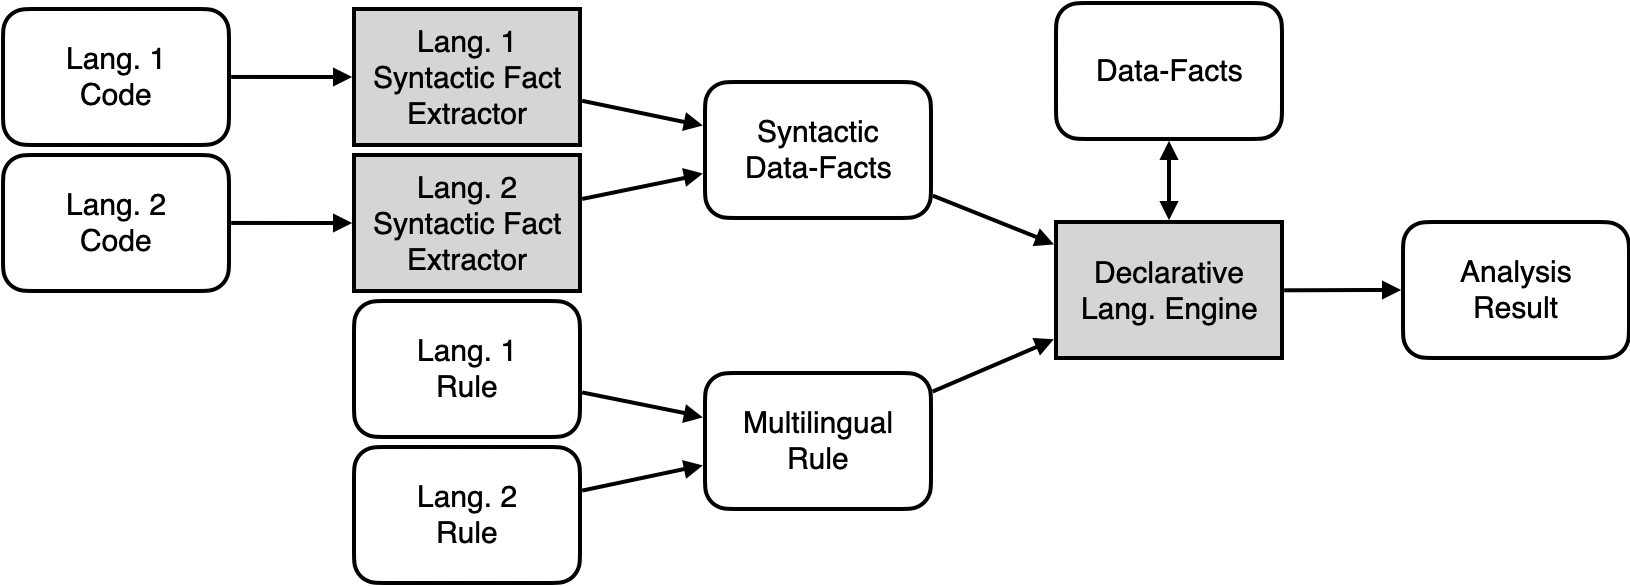
\includegraphics[width=0.47\textwidth]{img/overview}
%  \vspace*{-1.5em}
  \caption{Declarative analysis for monolingual programs}
  \label{fig:overview}
%\vspace*{-.5em}
\end{figure}

\section{Multilingual Program Analysis using Declarative Static Analyzers}
\label{sec:approach}

In this section, we propose a general approach to perform a declarative
static analysis for multilingual programs.

\subsection{Declarative Analysis for a Single Language}

A declarative analysis~\cite{doop} consists of datafacts and rules:
\[
  \begin{array}{llll}
d & ::= & p(\overline{e}) & \mbox{datafact}\\
e & ::= & \embox{num}~\mid~\embox{string} & \mbox{element}\\
r & ::= & d\ \mbox{:-}\ \overline{\neg^? d} & \mbox{rule}
\end{array}
\]
A datafact ``$d = p(\overline{e})$'' denotes a relation $p$ between elements $\overline{e}$.
An element $e$ is either a number or a string.
A rule ``$r = d'\ \mbox{:-}\ \overline{\neg^? d}$'' denotes that
a datafact $d'$ can be derived from other datafacts $\overline{d}$;
$d'$ holds if all the datafacts $d \in \{\overline{\neg^? d}\}$ hold
and all the datafacts $\neg d \in \{\overline{\neg^? d}\}$ does not hold.

Figure~\ref{fig:overview} presents the overview of how a
declarative-style analysis works for monolingual programs.
The analysis consists of three steps.
First, a given program gets converted into syntactic datafacts.
Second, the rules that generate new datafacts are defined, which
correspond to the implementation of the analysis.
Finally, a declarative language engine evaluates the rules with the given datafacts,
producing an analysis result in the form of a datafact.

\medskip
\textbf{Step 1: Extracting syntactic datafacts.}
The first step is to extract syntactic datafacts from a given source code.
Syntactic datafacts include datafacts about certain AST nodes and
the parent-child relationship between nodes. For example, consider
the following code:

\begin{lstlisting}[style=cpp,xleftmargin=2.5em]
int x = 42 + 43;
\end{lstlisting}
We can define a syntactic datafact of the form ``\datalog{expr(i, s)},''
where \datalog{i} denotes the expression ID and \datalog{s}
denotes a string representation of the expression in the source code.
Therefore, we can extract the following set of expr datafacts:
\datalog{expr(0, "42")}, \datalog{expr(1, "43")}, and \datalog{expr(2, "42 + 43")}.
They denote that \datalog{"42"} is the 0-th expression,
\datalog{"42"} is the first, and \datalog{"42 + 43"} is the second.
Another example syntactic datafact is ``\datalog{subexpr(i, j, k)},''
which denotes that the \datalog{i}-th expression has the \datalog{j}-th
expression as the \datalog{k}-th subexpression.
For example, we can extract the following syntactic datafacts:
\datalog{subexpr(2, 0, 0)} and \datalog{subexpr(2, 1, 1)}.

In a sense, these syntactic datafacts serve as building blocks for the
common Intermediate Representation (IR) of multiple languages.
Compared to other IRs, this declarative-style IR has a few advantages.
First, extracting information from source code in this format does not
require any consideration of the language semantics, which imposes
almost no performance overhead beyond parsing the source code.
Second, the syntactic datafacts can be utilized easily in any other kind of
analysis, since they are simple information that can be freely
manipulated by defining new rules. Therefore, even when we use a different
client analysis, we can reuse the extracted syntactic datafacts
without re-extracting them from the source code.


\medskip
\textbf{Step 2: Defining rules.}
The next step is to define rules to generate new datafacts out of known datafacts.
This step corresponds to actually implementing the algorithm of a
static analysis in a declarative style.
For example, recall that we can define a dataflow analysis
\datalog{flow(a, b)} as the transitive closure of the datafact
named \datalog{step}.
Then, we should define rules for the datafact \datalog{step}.
For example, if the syntactic datafact \datalog{assign(x, val)}
denotes the assignment \ccode{x = val}, then we can define a rule for
\datalog{step} and the assignment as follows:
\begin{lstlisting}[style=myDatalog,xleftmargin=2.5em]
step(a, b) :- assign(a, b)
\end{lstlisting}


% {\color{red}{To make this step applicable to multilingual analysis, we present
% a way to define rules in a ``framework approach.''
% First, we design a framework for a static analysis, which consists of 
% the result datafact which would correspond to the
% final result of the analysis, and some helper datafacts used for calculating the result datafact.
%  Then, second task is to actually fill in the rules for such helper datafacts.

% Let's look at the concrete example of dataflow analysis. First thing we do is
% designing the dataflow analysis framework.  In this framework, the final
% analysis result we want is expressed with the datafact of the form of
% flow(a,b), which means that value of the node a can flow into node b. flow(a,
% b) can be defined as transitive closure of a datafact \datalog{step(a, b)};

% \begin{lstlisting}[style=myDatalog,xleftmargin=2.5em]
% flow(a,b) :- step(a,b)
% flow(a,b) :- step(a,c), flow(c, b)
% \end{lstlisting}
% where the datafact step(a,b) means that there is a direct flow from node a to b.

% Next thing to do is defining rule for the helper datafact, step.  For example,
% let's assume that the syntactic datafact assign(x, val) indicates the assignment
% x = val, then one can define a rule for step to be
% \begin{lstlisting}[style=myDatalog,xleftmargin=2.5em]
% step(a,b) :- assign(a, b)
% \end{lstlisting}
% }}


\medskip
\textbf{Step 3: Evaluating rules.}
The final step is to simply evaluate the defined rules with the given datafacts.
Evaluating the rules amounts to finding all possible
datafacts that can be derived. The rules are usually evaluated in a bottom-up
and modular manner, that is, each rule is evaluated one-by-one, after every
rule it depends on is evaluated.

\begin{figure}[t]
  \centering
  \vspace{2mm}
  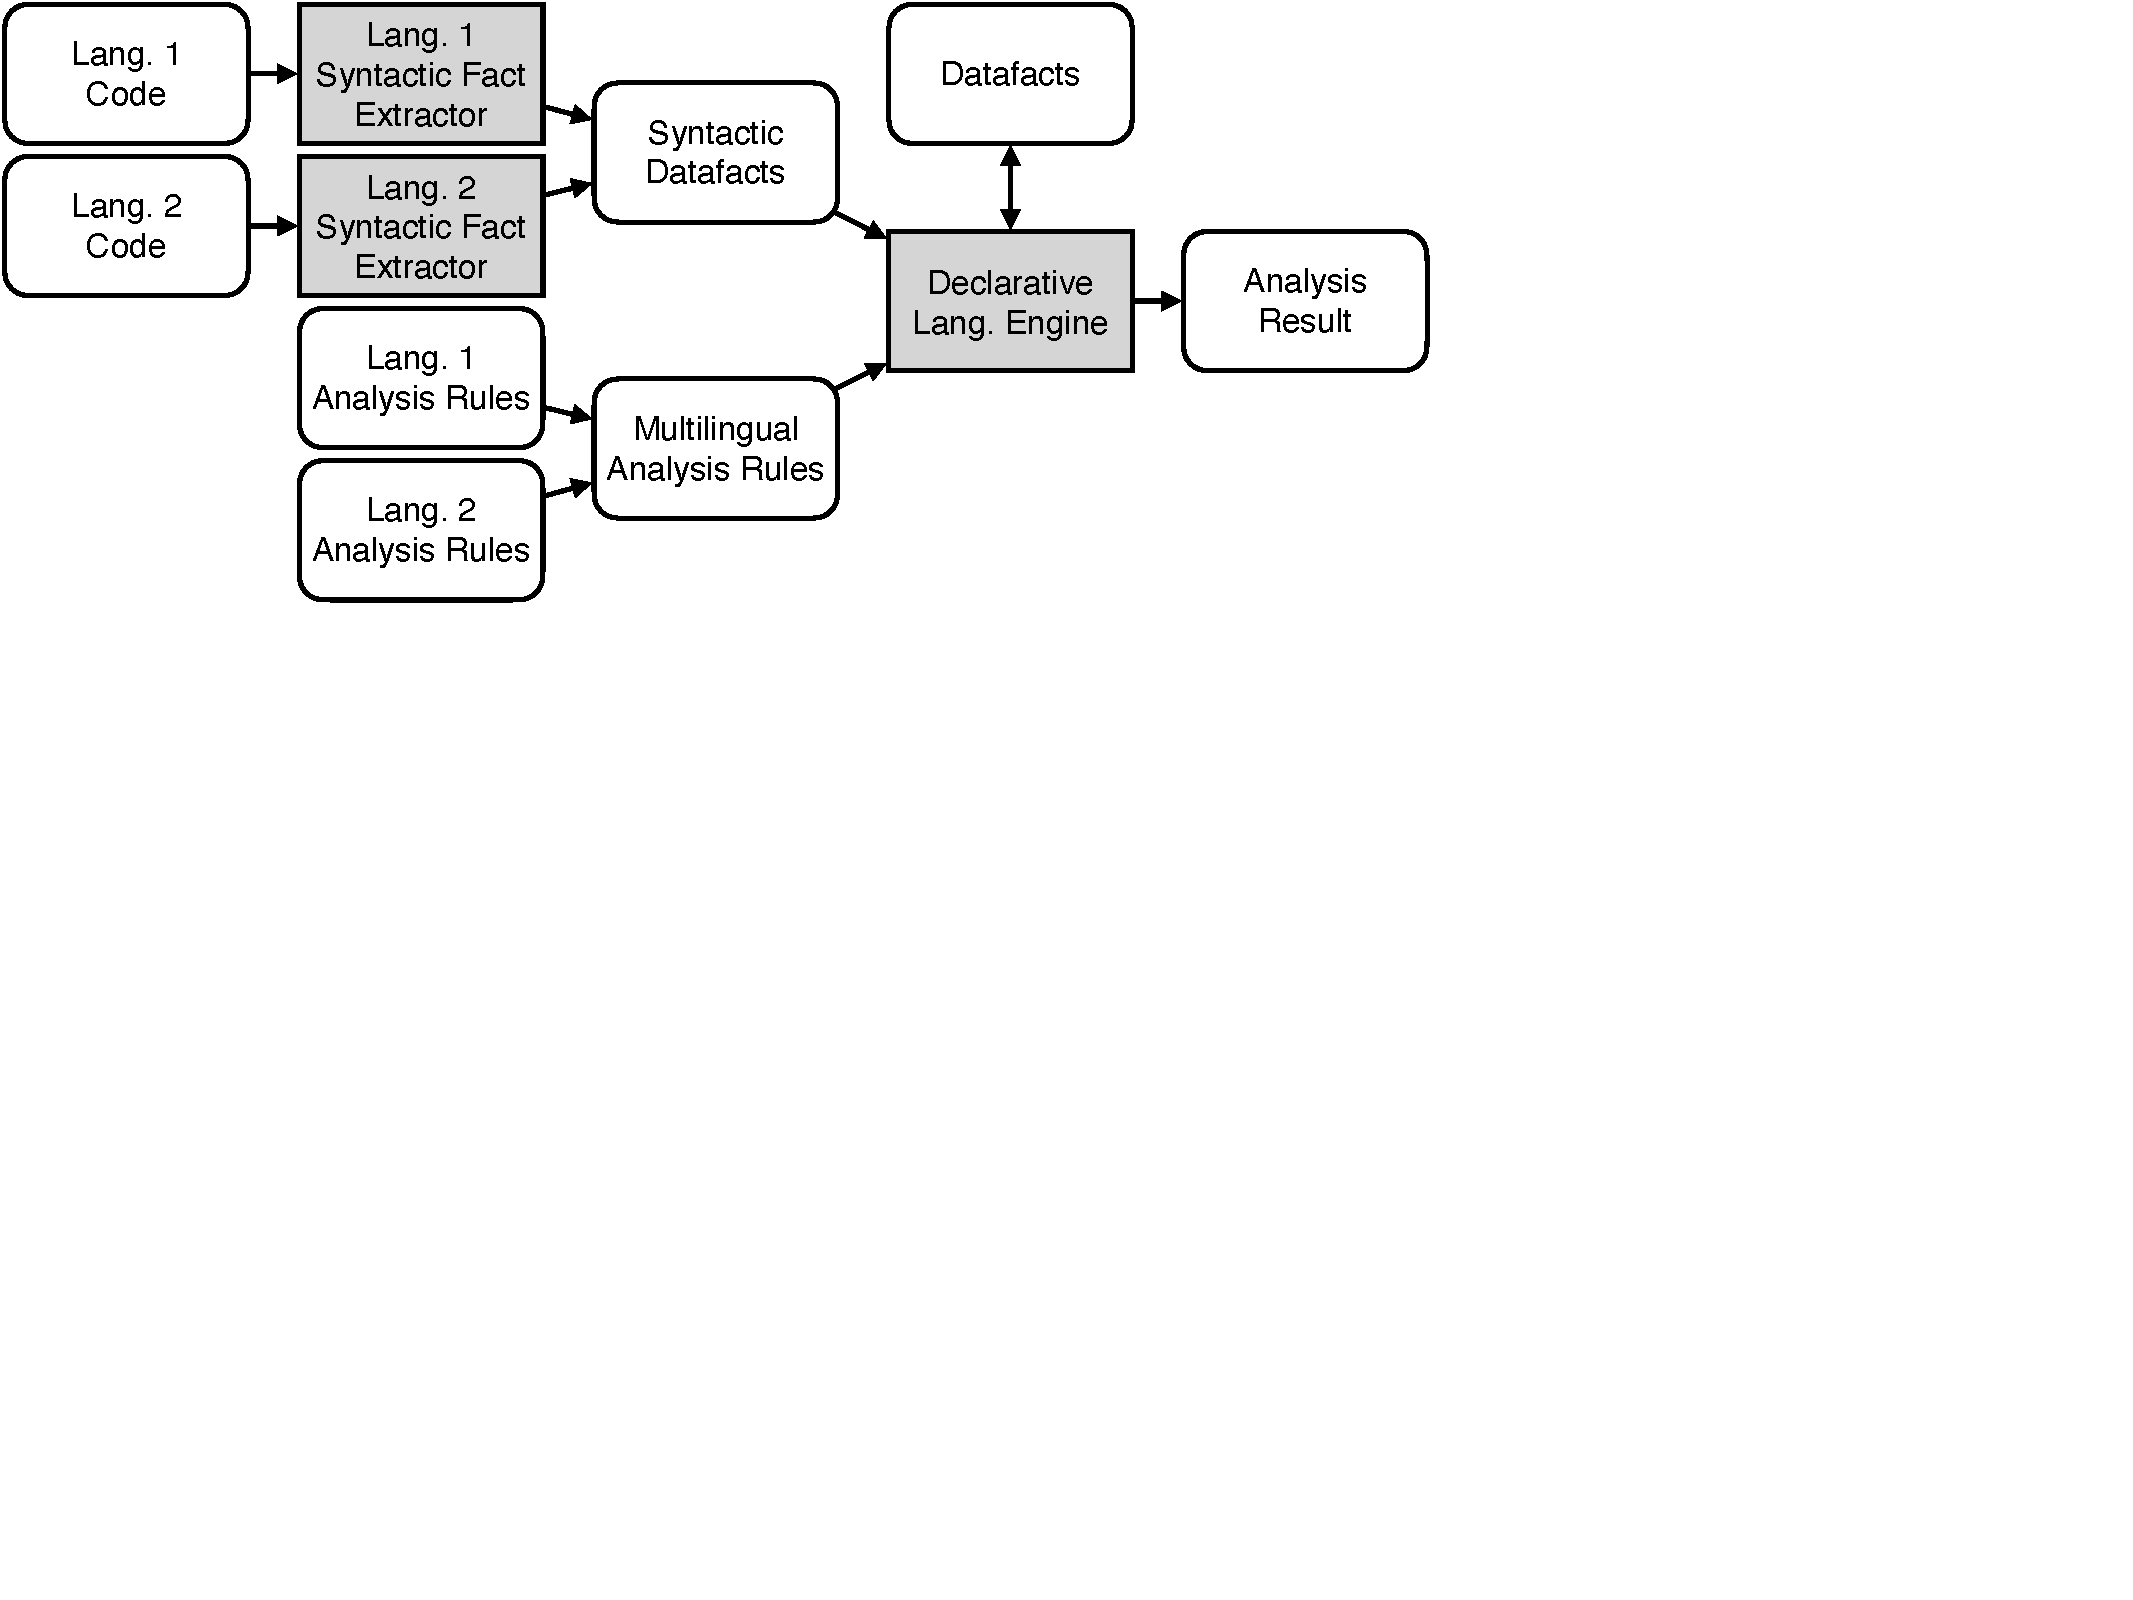
\includegraphics[width=0.47\textwidth]{img/overview2}
  \caption{Declarative analysis for multilingual programs}
  \label{fig:overview2}
%\vspace*{-.5em}
\end{figure}

\subsection{\mbox{Declarative Analysis for Multiple Languages}}
Now, we explain how we can compose two declarative-style static analyzers
for monolingual programs to perform analysis on multilingual programs.

Figure~\ref{fig:overview2} illustrates how we support multilingual
analysis in a declarative style in the case of two languages as an
example. The declarative language engine now gets two sets of
syntactic datafacts extracted from different languages. In addition,
the rules from different languages are also merged, taking the
interoperation semantics into account by extending corresponding
rules.

To merge sets of rules from multiple languages easily,
the rules from multiple languages should share ``common datafacts and rules''
that exist in each language. While each language shares the same set of
common datafacts and rules, the rules for deriving them may differ in different languages.
Given sets of rules for multiple programming languages,
we first identify syntactic parts of a given program where
interactions between different languages can happen.
Then, using this interoperation information,
we define new rules generating necessary datafacts to model
the interoperation semantics.
One thing to note here is that pre-defined intra-language rules for common
datafacts and newly-defined inter-language rules can be treated independently;
we can define new rules without considering or modifying existing
implementation.

Let us revisit the dataflow analysis example for multilingual programs
writtin in the language A and the language B.
First, we merge each set of rules from each language.
For example, we merge the rules for the datafact \datalog{step} from each language:
\begin{lstlisting}[style=myDatalog,xleftmargin=2.5em]
step(a, b) :- step_A(a, b)
step(a, b) :- step_B(a, b)
\end{lstlisting}
To take inter-language dataflows into account, we should also specify
how a data of one language can be passed to another language cross language
boundaries.  For example, one can pass data in one language into
another by a function call as shown below:

\begin{lstlisting}[style=java,xleftmargin=2.5em]
public void main() { // Language A
  int x = SOURCE();
  B::f(x);
}
void f(int param) {  // Language B
  printf("\%d", param);
}
\end{lstlisting}
The variable \javacode{x} in the language A is passed to the parameter
of a function \javacode{f} in the language B.  To reflect such a data flow,
we can define the datafact \datalog{foreignArgParam(a, b, i)},
which denotes that \datalog{a} is the \datalog{i}-th argument of a foreign
function call to a function whose \datalog{i}-th parameter is \datalog{b}.
From the above example, we can derive the datafact \datalog{foreignArgParam(x, param, 0)}.
Using this datafact, we can add a new rule to derive the common datafact
\datalog{step} as follows:
\begin{lstlisting}[style=myDatalog,xleftmargin=2.5em]
step(a, b) :- foreignArgParam(a, b, i)
\end{lstlisting}
which enables dataflows via foreign function calls cross language boundaries.
